\documentclass[11pt]{article}

\usepackage{pablo}
\usepackage{yhmath}
\usepackage{multicol}
\usetikzlibrary{trees}
\usetikzlibrary{arrows}
\usetikzlibrary{positioning,backgrounds}

\usepackage[a5paper,margin=1.4cm]{geometry}

\pagestyle{empty}
\begin{document}

\begin{center}
  \textsc{DM}
  ---
  {
    \Large
    Probabilités
  }

    \textsc{Correction}

    ~
    \hrule
\end{center}

\begin{exercice}
  \begin{em}
    J'ai écrit un programme sur ma calculatrice, qui affiche aléatoirement un des nombres 0, 1, 2 ou 3. On connait les probabilités suivantes :
    \begin{itemize}
      \item le nombre affiché est pair : $^5/_6$ ;
      \item le nombre affiché est strictement positif : $^3/_4$ ;
      \item le nombre affiché est 3 : $^1/_6$.
    \end{itemize}
    Quelle est la probabilité d'obtenir 1 ?
  \end{em}

    On va compléter une partie du tableau suivant.

  \begin{center}\begin{tabular}{l|c|c|c|c}
    Nombre & 0 & 1 & 2 & 3 \\
    \hline
    Probabilité & $p_0$ & $p_1$ & $p_2$ & $p_3$
  \end{tabular}\end{center}

  On sait que la probabilité d'obtenir un nombre pair est $^5/_6$, donc la probabilité d'obtenir un nombre impair est $1-\frac{5}{6}=\frac{1}{6}$.

  L'évènement « Obtenir un nombre impair » est constitué des évènements « Obtenir 1 » et « Obtenir 3 ». De plus, ces deux évènements sont incompatibles, donc $P(\text{« Obtenir un nombre impair »}) = p_1 + p_3$. Or, $p_3=\frac{1}{6}$, donc $p_1=P(\text{« Obtenir un nombre impair »}) - p_3=\frac{1}{6}-\frac{1}{6}=0$.

La probabilité d'obtenir 1 est donc nulle.

\emph{On remarque que nous n'avons pas utilisé ici la probabilité d'obtenir un nombre positif. Il était aussi possible de faire avec.}


\end{exercice}

\begin{exercice}
  \begin{em}
  Une urne contient quatre boules indiscernables au toucher, numérotées de 1 à 4. On tire successivement deux boules, sans remise.
  \begin{enumerate}
    \item Donner la taille de l'univers de cette expérience aléatoire.
    \item Quelle est la probabilité que la seconde boule porte un numéro plus grand que la première ?
    \item Quelle est la probabilité que la somme des deux boules fasse 4 ?
  \end{enumerate}
\end{em}

\newpage
  \begin{multicols}{2}
  \begin{center}
      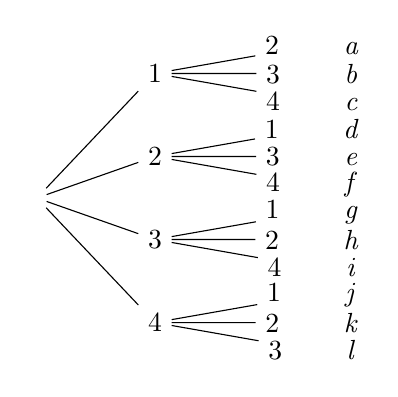
\begin{tikzpicture}[grow=right, sloped]
        % Set the overall layout of the tree
        \tikzstyle{level 1}=[level distance=1.5cm, sibling distance=3em]
        \tikzstyle{level 2}=[level distance=2cm, sibling distance=1em]
        \node {}
        child {
          node {4}
          child {
            node {3 \hspace{2em}\emph{l}}
            edge from parent
          }
          child {
            node {2 \hspace{2em}\emph{k}}
            edge from parent
          }
          child {
            node {1 \hspace{2em}\emph{j}}
            edge from parent
          }
          edge from parent
        }
        child {
          node {3}
          child {
            node {4 \hspace{2em}\emph{i}}
            edge from parent
          }
          child {
            node {2 \hspace{2em}\emph{h}}
            edge from parent
          }
          child {
            node {1 \hspace{2em}\emph{g}}
            edge from parent
          }
          edge from parent
        }
        child {
          node {2}
          child {
            node {4 \hspace{2em}\emph{f}}
            edge from parent
          }
          child {
            node {3 \hspace{2em}\emph{e}}
            edge from parent
          }
          child {
            node {1 \hspace{2em}\emph{d}}
            edge from parent
          }
          edge from parent
        }
        child {
          node {1}
          child {
            node {4 \hspace{2em}\emph{c}}
            edge from parent
          }
          child {
            node {3 \hspace{2em}\emph{b}}
            edge from parent
          }
          child {
            node {2 \hspace{2em}\emph{a}}
            edge from parent
          }
          edge from parent
        };
      \end{tikzpicture}
    \end{center}

    L'arbre correspondant à cette expérience est représenté ci-contre ; chaque branche est repérée par une lettre. Pour ne pas le surcharger, nous n'avons pas inscrit les probabilités de chaque branche, mais les issues sont équiprobables : la probabilité de chaque branche de la première expérience est $^1/_4$, et la probabilité de chaque branche de la seconde expérience est $^1/_3$.
  \end{multicols}

  \begin{enumerate}
    \item La taille de l'univers est le nombre de « feuilles » (de branches terminales) de l'arbre. Il y en a 12.
    \item Les branches correspondant à cette évènement sont les branches $a$, $b$, $c$, $e$, $f$, $i$. Chacune a une probabilité de $\frac{1}{4}\times\frac{1}{3}=\frac{1}{12}$, donc l'évènement a une probabilité de $6\times\frac{1}{12}=\frac{1}{2}$.
    \item Les branches correspondant à cette évènement sont les branches $b$ et $g$. Avec le même raisonnement, on trouve une probabilité de $2\times\frac{1}{12}=\frac{1}{6}$.
  \end{enumerate}
\end{exercice}

\begin{exercice}
  \begin{em}
    \begin{enumerate}
      \item On lance une pièce de monnaie deux fois de suite. Cette pièce est mal équilibrée : il y a une chance sur trois de faire pile, et deux chances sur trois de faire face.
        \begin{enumerate}
          \item Combien y a-t-il d'issues à cette expérience aléatoire ?
          \item Soit $A$ l'évènement « obtenir deux fois pile ». Déterminer $P(A)$.
          \item Soit $B$ l'évènement « obtenir exactement une fois face ». Déterminer $P(B)$.
          \item Décrire $\bar B$. Calculer sa probabilité.
        \end{enumerate}
      \item On lance deux pièces de monnaie indistinguables, donnant pile et face avec les mêmes probabilités que la pièce de la question précédente. Répondre aux même questions que pour la première expérience.
    \end{enumerate}
  \end{em}

  \newpage

  \begin{enumerate}
    \item~
      \begin{multicols}{2}
        \begin{center}
          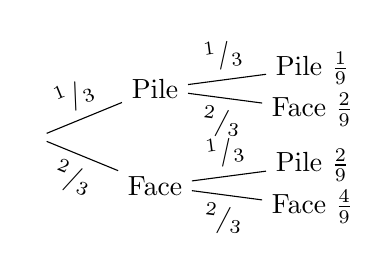
\begin{tikzpicture}[grow=right, sloped]
            % Set the overall layout of the tree
            \tikzstyle{level 1}=[level distance=1.5cm, sibling distance=3.5em]
            \tikzstyle{level 2}=[level distance=2cm, sibling distance=1.5em]
            \node {}
            child {
              node {Face}
              child {
                node {Face $\frac{4}{9}$}
                edge from parent
                node[midway,below]{$^2/_3$}
              }
              child {
                node {Pile $\frac{2}{9}$}
                edge from parent
                node[midway,above]{$^1/_3$}
              }
              edge from parent
              node[midway,below]{$^2/_3$}
            }
            child {
              node {Pile}
              child {
                node {Face $\frac{2}{9}$}
                edge from parent
                node[midway,below]{$^2/_3$}
              }
              child {
                node {Pile $\frac{1}{9}$}
                edge from parent
                node[midway,above]{$^1/_3$}
              }
              edge from parent
              node[midway,above]{$^1/_3$}
            };
          \end{tikzpicture}
        \end{center}

        L'arbre correspondant à cette expérience est représenté ci-contre. La probabilité de chaque branche est affichée sur sa droite.
      \end{multicols}
      \begin{enumerate}
        \item Le nombre d'issues est le nombre de « feuilles » de l'arbre : il y en a quatre.
        \item Seule la première branche correspond à l'évènement « obtenir deux fois piles ». Sa probabilité est donc $^1/_9$.
        \item Les deuxième et troisième branches correspondent à l'évènement « obtenir exactement une fois face ». La probabilité de cet évènement est donc la somme des probabilités de ces deux branches, soit $\frac{2}{9}+\frac{2}{9}=\frac{4}{9}$.
        \item $\bar B$ est le contraire de l'évènement « Obtenir exactement une fois face ». On peut donc le décrire comme « Ne pas obtenir exactement une fois face », ou encore « Obtenir zéro ou deux faces ». Sa probabilité est $1-P(B)=1-\frac{4}{9}=\frac{5}{9}$.
      \end{enumerate}
    \item On utilise le même arbre pour représenter les expériences aléatoires correspondant aux lancers successifs de la même pièce, ou au lancer simultané de deux pièces identiques. Donc les réponses à cette question sont les mêmes que celles de la question précédente.
  \end{enumerate}
\end{exercice}

\end{document}
